\documentclass[crop,tikz]{standalone}
\usepackage{amsmath}
\usepackage{amsfonts}
\usepackage{physics}
\usepackage{tikz}
\usetikzlibrary{shapes}
\usepackage{dsfont}
\usepackage{bbm}
% parameters for the MPS drawings
\definecolor{Tcolor}{RGB}{255, 235, 171}
\definecolor{Wcolor}{RGB}{190, 190, 255}
\def\textoffsetVertical{0.8}
\def\nodewidth{0.6*28.5}
\def\legwidth{0.8}
\def\nodedistance{1.25}
\def\textoffsetVerticalW{0.9}
\def\textoffsetHorizontalW{-0.9}
\def\textoffsetVerticalMPO{1.2}
\def\yoffset{1}
\def\xoffset{3}
\def\resultMPSYoffset{2.5}
\def\resultMPSXOffsetSmall{2}
\def\resultMPSXOffset{3}
\def\dotsOffset{3}
\def\conjOffsetVertical{1.25}
\def\conjOffsetVerticalLarge{2.2}
\def\curvedLineXOffset{0.7}
\def\cmscale{28.5}
\def\miniatureScale{0.5}
\def\Heffheight{1.2*28.5}
\def\Heffwidth{4.0*28.5}
\def\Heffonewidth{3.0*28.5}
\def\miniatureTextOffsetVertical{0.5}
\begin{document}
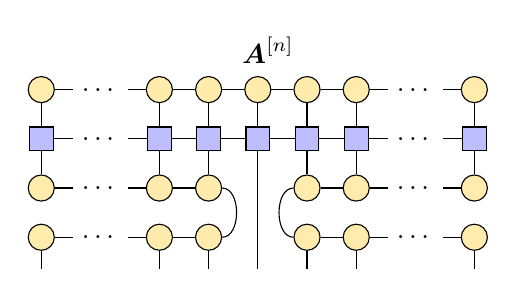
\begin{tikzpicture}[baseline=(current  bounding  box.center)]
    \node[draw, shape=circle, fill=Tcolor, minimum width=\nodewidth*\miniatureScale] (T1) at (0, 0) {};
    \node[draw, shape=circle, fill=Tcolor, minimum width=\nodewidth*\miniatureScale] (T2) at ({(1*\dotsOffset)*\miniatureScale}, 0) {};
    \node[draw, shape=circle, fill=Tcolor, minimum width=\nodewidth*\miniatureScale] (T3) at ({(1*\nodedistance+1*\dotsOffset)*\miniatureScale}, 0) {};
    \node[draw, shape=circle, fill=Tcolor, minimum width=\nodewidth*\miniatureScale] (T4) at ({(3*\nodedistance+1*\dotsOffset)*\miniatureScale}, 0) {};
    \node[draw, shape=circle, fill=Tcolor, minimum width=\nodewidth*\miniatureScale] (T5) at ({(4*\nodedistance+1*\dotsOffset)*\miniatureScale}, 0) {};
    \node[draw, shape=circle, fill=Tcolor, minimum width=\nodewidth*\miniatureScale] (T6) at ({(4*\nodedistance+2*\dotsOffset)*\miniatureScale}, 0) {};

    \node[draw, shape=circle, fill=Tcolor, minimum width=\nodewidth*\miniatureScale] (T1c) at (0, -\conjOffsetVertical*\miniatureScale) {};
    \node[draw, shape=circle, fill=Tcolor, minimum width=\nodewidth*\miniatureScale] (T2c) at ({(1*\dotsOffset)*\miniatureScale}, -\conjOffsetVertical*\miniatureScale) {};
    \node[draw, shape=circle, fill=Tcolor, minimum width=\nodewidth*\miniatureScale] (T3c) at ({(1*\nodedistance+1*\dotsOffset)*\miniatureScale}, -\conjOffsetVertical*\miniatureScale) {};
    \node[draw, shape=circle, fill=Tcolor, minimum width=\nodewidth*\miniatureScale] (T4c) at ({(3*\nodedistance+1*\dotsOffset)*\miniatureScale}, -\conjOffsetVertical*\miniatureScale) {};
    \node[draw, shape=circle, fill=Tcolor, minimum width=\nodewidth*\miniatureScale] (T5c) at ({(4*\nodedistance+1*\dotsOffset)*\miniatureScale}, -\conjOffsetVertical*\miniatureScale) {};
    \node[draw, shape=circle, fill=Tcolor, minimum width=\nodewidth*\miniatureScale] (T6c) at ({(4*\nodedistance+2*\dotsOffset)*\miniatureScale}, -\conjOffsetVertical*\miniatureScale) {};

    \draw (T1) -- ++(\legwidth*\miniatureScale, 0);
    \draw (T2) -- ++(-\legwidth*\miniatureScale, 0);
    \draw (T2) -- (T3);
    \draw (T4) -- (T5);
    \draw (T5) -- ++(\legwidth*\miniatureScale, 0);
    \draw (T6) -- ++(-\legwidth*\miniatureScale, 0);

    \draw (T1c) -- ++(\legwidth*\miniatureScale, 0);
    \draw (T1c) -- ++(0, -\legwidth*\miniatureScale);
    \draw (T2c) -- ++(-\legwidth*\miniatureScale, 0);
    \draw (T2c) -- ++(0, -\legwidth*\miniatureScale);
    \draw (T2c) -- (T3c);
    \draw (T3c) -- ++(0, -\legwidth*\miniatureScale);
    \draw (T4c) -- (T5c);
    \draw (T4c) -- ++(0, -\legwidth*\miniatureScale);
    \draw (T5c) -- ++(0, -\legwidth*\miniatureScale);
    \draw (T5c) -- ++(\legwidth*\miniatureScale, 0);
    \draw (T6c) -- ++(0, -\legwidth*\miniatureScale);
    \draw (T6c) -- ++(-\legwidth*\miniatureScale, 0);

    \draw (T3) to[in=0, out=0, looseness = 1] (T3c);
    \draw (T4) to[in=180, out=180, looseness = 1] (T4c);

    \node[] (dots1) at (\dotsOffset/2*\miniatureScale, 0) {$\dots$};
    \node[] (dots1) at (\dotsOffset/2*\miniatureScale, -\conjOffsetVertical*\miniatureScale) {$\dots$};
    \node[] (dots1) at ({(4*\nodedistance+1.5*\dotsOffset)*\miniatureScale}, 0) {$\dots$};
    \node[] (dots1) at ({(4*\nodedistance+1.5*\dotsOffset)*\miniatureScale}, -\conjOffsetVertical*\miniatureScale) {$\dots$};

    % MPO
    \node[draw, shape=rectangle, fill=Wcolor, minimum width=\nodewidth*\miniatureScale, minimum height=\nodewidth*\miniatureScale] (W1) at (0, \conjOffsetVertical*\miniatureScale) {};
    \node[draw, shape=rectangle, fill=Wcolor, minimum width=\nodewidth*\miniatureScale, minimum height=\nodewidth*\miniatureScale] (W2) at ({(1*\dotsOffset)*\miniatureScale}, \conjOffsetVertical*\miniatureScale) {};
    \node[draw, shape=rectangle, fill=Wcolor, minimum width=\nodewidth*\miniatureScale, minimum height=\nodewidth*\miniatureScale] (W3) at ({(1*\nodedistance+1*\dotsOffset)*\miniatureScale}, \conjOffsetVertical*\miniatureScale) {};
    \node[draw, shape=rectangle, fill=Wcolor, minimum width=\nodewidth*\miniatureScale, minimum height=\nodewidth*\miniatureScale] (W4) at ({(2*\nodedistance+1*\dotsOffset)*\miniatureScale}, \conjOffsetVertical*\miniatureScale) {};
    \node[draw, shape=rectangle, fill=Wcolor, minimum width=\nodewidth*\miniatureScale, minimum height=\nodewidth*\miniatureScale] (W5) at ({(3*\nodedistance+1*\dotsOffset)*\miniatureScale}, \conjOffsetVertical*\miniatureScale) {};
    \node[draw, shape=rectangle, fill=Wcolor, minimum width=\nodewidth*\miniatureScale, minimum height=\nodewidth*\miniatureScale] (W6) at ({(4*\nodedistance+1*\dotsOffset)*\miniatureScale}, \conjOffsetVertical*\miniatureScale) {};
    \node[draw, shape=rectangle, fill=Wcolor, minimum width=\nodewidth*\miniatureScale, minimum height=\nodewidth*\miniatureScale] (W7) at ({(4*\nodedistance+2*\dotsOffset)*\miniatureScale}, \conjOffsetVertical*\miniatureScale) {};

    \draw (W1) -- (T1);
    \draw (W2) -- (T2);
    \draw (W3) -- (T3);
    \draw (W5) -- (T4);
    \draw (W6) -- (T5);
    \draw (W7) -- (T6);

    \draw (W4) -- ++(0, {(-2*\conjOffsetVertical-\legwidth)*\miniatureScale});

    \draw (W2) -- (W3) -- (W4) -- (W5) -- (W6);

    \draw (W1) -- ++(\legwidth*\miniatureScale, 0);
    \draw (W6) -- ++(\legwidth*\miniatureScale, 0);
    \draw (W2) -- ++(-\legwidth*\miniatureScale, 0);
    \draw (W7) -- ++(-\legwidth*\miniatureScale, 0);

    \node[] (dots1) at (\dotsOffset/2*\miniatureScale, \conjOffsetVertical*\miniatureScale) {$\dots$};
    \node[] (dots1) at ({(4*\nodedistance+1.5*\dotsOffset)*\miniatureScale}, \conjOffsetVertical*\miniatureScale) {$\dots$};

    % MPS on top
    \node[draw, shape=circle, fill=Tcolor, minimum width=\nodewidth*\miniatureScale] (T1) at (0, 2*\conjOffsetVertical*\miniatureScale) {};
    \node[draw, shape=circle, fill=Tcolor, minimum width=\nodewidth*\miniatureScale] (T2) at ({(1*\dotsOffset)*\miniatureScale}, 2*\conjOffsetVertical*\miniatureScale) {};
    \node[draw, shape=circle, fill=Tcolor, minimum width=\nodewidth*\miniatureScale] (T3) at ({(1*\nodedistance+1*\dotsOffset)*\miniatureScale}, 2*\conjOffsetVertical*\miniatureScale) {};
    \node[draw, shape=circle, fill=Tcolor, minimum width=\nodewidth*\miniatureScale] (T4) at ({(2*\nodedistance+1*\dotsOffset)*\miniatureScale}, 2*\conjOffsetVertical*\miniatureScale) {};
    \node[draw, shape=circle, fill=Tcolor, minimum width=\nodewidth*\miniatureScale] (T5) at ({(3*\nodedistance+1*\dotsOffset)*\miniatureScale}, 2*\conjOffsetVertical*\miniatureScale) {};
    \node[draw, shape=circle, fill=Tcolor, minimum width=\nodewidth*\miniatureScale] (T6) at ({(4*\nodedistance+1*\dotsOffset)*\miniatureScale}, 2*\conjOffsetVertical*\miniatureScale) {};
    \node[draw, shape=circle, fill=Tcolor, minimum width=\nodewidth*\miniatureScale] (T7) at ({(4*\nodedistance+2*\dotsOffset)*\miniatureScale}, 02*\conjOffsetVertical*\miniatureScale) {};

    \draw (W1) -- (T1);
    \draw (W2) -- (T2);
    \draw (W3) -- (T3);
    \draw (W4) -- (T4);
    \draw (W5) -- (T5);
    \draw (W6) -- (T6);
    \draw (W7) -- (T7);

    \draw (T2) -- (T3) -- (T4) -- (T5) -- (T6);

    \draw (T1) -- ++(\legwidth*\miniatureScale, 0);
    \draw (T6) -- ++(\legwidth*\miniatureScale, 0);
    \draw (T2) -- ++(-\legwidth*\miniatureScale, 0);
    \draw (T7) -- ++(-\legwidth*\miniatureScale, 0);

    \node[] (dots1) at (\dotsOffset/2*\miniatureScale, 2*\conjOffsetVertical*\miniatureScale) {$\dots$};
    \node[] (dots1) at ({(4*\nodedistance+1.5*\dotsOffset)*\miniatureScale}, 2*\conjOffsetVertical*\miniatureScale) {$\dots$};

    \node[] (thetatext) at ({(2*\nodedistance+1*\dotsOffset)*\miniatureScale+0.13}, 2*\conjOffsetVertical*\miniatureScale+\miniatureTextOffsetVertical) {$\vb*{A}^{[n]}$};

\end{tikzpicture}
\end{document}